%% Creator: Inkscape inkscape 0.92.2, www.inkscape.org
%% PDF/EPS/PS + LaTeX output extension by Johan Engelen, 2010
%% Accompanies image file 'fle41.eps' (pdf, eps, ps)
%%
%% To include the image in your LaTeX document, write
%%   \input{<filename>.pdf_tex}
%%  instead of
%%   \includegraphics{<filename>.pdf}
%% To scale the image, write
%%   \def\svgwidth{<desired width>}
%%   \input{<filename>.pdf_tex}
%%  instead of
%%   \includegraphics[width=<desired width>]{<filename>.pdf}
%%
%% Images with a different path to the parent latex file can
%% be accessed with the `import' package (which may need to be
%% installed) using
%%   \usepackage{import}
%% in the preamble, and then including the image with
%%   \import{<path to file>}{<filename>.pdf_tex}
%% Alternatively, one can specify
%%   \graphicspath{{<path to file>/}}
%% 
%% For more information, please see info/svg-inkscape on CTAN:
%%   http://tug.ctan.org/tex-archive/info/svg-inkscape
%%
\begingroup%
  \makeatletter%
  \providecommand\color[2][]{%
    \errmessage{(Inkscape) Color is used for the text in Inkscape, but the package 'color.sty' is not loaded}%
    \renewcommand\color[2][]{}%
  }%
  \providecommand\transparent[1]{%
    \errmessage{(Inkscape) Transparency is used (non-zero) for the text in Inkscape, but the package 'transparent.sty' is not loaded}%
    \renewcommand\transparent[1]{}%
  }%
  \providecommand\rotatebox[2]{#2}%
  \ifx\svgwidth\undefined%
    \setlength{\unitlength}{602.31990694bp}%
    \ifx\svgscale\undefined%
      \relax%
    \else%
      \setlength{\unitlength}{\unitlength * \real{\svgscale}}%
    \fi%
  \else%
    \setlength{\unitlength}{\svgwidth}%
  \fi%
  \global\let\svgwidth\undefined%
  \global\let\svgscale\undefined%
  \makeatother%
  \begin{picture}(1,0.56554637)%
    \put(0,0){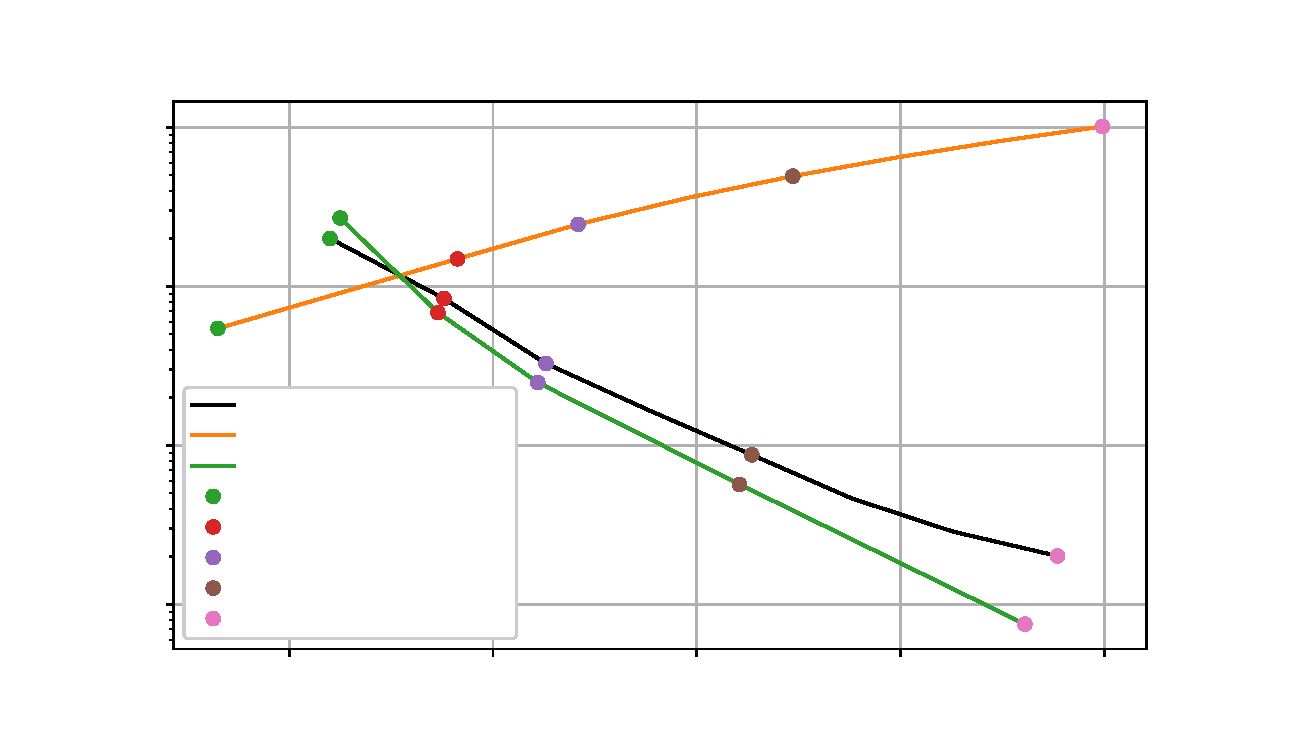
\includegraphics[width=\unitlength]{images_2ddl/fle41.eps}}%
    \put(0.20661598,0.03809743){\color[rgb]{0,0,0}\makebox(0,0)[lb]{\smash{10}}}%
    \put(0.36902801,0.03809743){\color[rgb]{0,0,0}\makebox(0,0)[lb]{\smash{20}}}%
    \put(0.53144004,0.03809743){\color[rgb]{0,0,0}\makebox(0,0)[lb]{\smash{30}}}%
    \put(0.69385207,0.03809743){\color[rgb]{0,0,0}\makebox(0,0)[lb]{\smash{40}}}%
    \put(0.85626575,0.03809743){\color[rgb]{0,0,0}\makebox(0,0)[lb]{\smash{50}}}%
    \put(0.067359896,0.09206078){\color[rgb]{0,0,0}\makebox(0,0)[lb]{\smash{$10^{-2}$}}}%
    \put(0.067359896,0.21808816){\color[rgb]{0,0,0}\makebox(0,0)[lb]{\smash{$10^{-1}$}}}%
    \put(0.078356045,0.34548557){\color[rgb]{0,0,0}\makebox(0,0)[lb]{\smash{$10^0$}}}%
    \put(0.078356045,0.47151162){\color[rgb]{0,0,0}\makebox(0,0)[lb]{\smash{$10^1$}}}%
    \put(0.06304079,0.23476368){\color[rgb]{0,0,0}\rotatebox{90}{\makebox(0,0)[lb]{\smash{$H_{ma x}(m)$}}}}%
    \put(0.5,0.01){\color[rgb]{0,0,0}\makebox(0,0)[lb]{\smash{$r_1 (mm)$}}}%
    \put(0.188649545,0.25123168){\color[rgb]{0,0,0}\makebox(0,0)[lb]{\smash{\scriptsize flambement/écoulement}}}%
    \put(0.18649545,0.22687253){\color[rgb]{0,0,0}\makebox(0,0)[lb]{\smash{\footnotesize $\delta/R>0.1$}}}%
    \put(0.18649545,0.20251338){\color[rgb]{0,0,0}\makebox(0,0)[lb]{\smash{\scriptsize écrasement de section}}}%
    \put(0.18649545,0.17815423){\color[rgb]{0,0,0}\makebox(0,0)[lb]{\smash{\footnotesize $r_2=15 mm$}}}%
    \put(0.18649545,0.15379592){\color[rgb]{0,0,0}\makebox(0,0)[lb]{\smash{\footnotesize $r_2=20 mm$}}}%
    \put(0.18649545,0.1294371){\color[rgb]{0,0,0}\makebox(0,0)[lb]{\smash{\footnotesize $r_2=25 mm$}}}%
    \put(0.18649545,0.10507812){\color[rgb]{0,0,0}\makebox(0,0)[lb]{\smash{\footnotesize $r_2=35 mm$}}}%
    \put(0.18649545,0.08071914){\color[rgb]{0,0,0}\makebox(0,0)[lb]{\smash{\footnotesize $r_2=50 mm$}}}%
  \end{picture}%
\endgroup%
